\documentclass[11pt,compress,t,notes=noshow, xcolor=table]{beamer}
\usepackage[]{graphicx}\usepackage[]{color}
% maxwidth is the original width if it is less than linewidth
% otherwise use linewidth (to make sure the graphics do not exceed the margin)
\makeatletter
\def\maxwidth{ %
  \ifdim\Gin@nat@width>\linewidth
    \linewidth
  \else
    \Gin@nat@width
  \fi
}
\makeatother

\definecolor{fgcolor}{rgb}{0.345, 0.345, 0.345}
\newcommand{\hlnum}[1]{\textcolor[rgb]{0.686,0.059,0.569}{#1}}%
\newcommand{\hlstr}[1]{\textcolor[rgb]{0.192,0.494,0.8}{#1}}%
\newcommand{\hlcom}[1]{\textcolor[rgb]{0.678,0.584,0.686}{\textit{#1}}}%
\newcommand{\hlopt}[1]{\textcolor[rgb]{0,0,0}{#1}}%
\newcommand{\hlstd}[1]{\textcolor[rgb]{0.345,0.345,0.345}{#1}}%
\newcommand{\hlkwa}[1]{\textcolor[rgb]{0.161,0.373,0.58}{\textbf{#1}}}%
\newcommand{\hlkwb}[1]{\textcolor[rgb]{0.69,0.353,0.396}{#1}}%
\newcommand{\hlkwc}[1]{\textcolor[rgb]{0.333,0.667,0.333}{#1}}%
\newcommand{\hlkwd}[1]{\textcolor[rgb]{0.737,0.353,0.396}{\textbf{#1}}}%
\let\hlipl\hlkwb

\usepackage{framed}
\makeatletter
\newenvironment{kframe}{%
 \def\at@end@of@kframe{}%
 \ifinner\ifhmode%
  \def\at@end@of@kframe{\end{minipage}}%
  \begin{minipage}{\columnwidth}%
 \fi\fi%
 \def\FrameCommand##1{\hskip\@totalleftmargin \hskip-\fboxsep
 \colorbox{shadecolor}{##1}\hskip-\fboxsep
     % There is no \\@totalrightmargin, so:
     \hskip-\linewidth \hskip-\@totalleftmargin \hskip\columnwidth}%
 \MakeFramed {\advance\hsize-\width
   \@totalleftmargin\z@ \linewidth\hsize
   \@setminipage}}%
 {\par\unskip\endMakeFramed%
 \at@end@of@kframe}
\makeatother

\definecolor{shadecolor}{rgb}{.97, .97, .97}
\definecolor{messagecolor}{rgb}{0, 0, 0}
\definecolor{warningcolor}{rgb}{1, 0, 1}
\definecolor{errorcolor}{rgb}{1, 0, 0}
\newenvironment{knitrout}{}{} % an empty environment to be redefined in TeX

\usepackage{alltt}
\newcommand{\SweaveOpts}[1]{}  % do not interfere with LaTeX
\newcommand{\SweaveInput}[1]{} % because they are not real TeX commands
\newcommand{\Sexpr}[1]{}       % will only be parsed by R
\newcommand{\xmark}{\ding{55}}%


\usepackage[english]{babel}
\usepackage[utf8]{inputenc}

\usepackage{dsfont}
\usepackage{verbatim}
\usepackage{amsmath}
\usepackage{amsfonts}
\usepackage{amssymb}
\usepackage{bm}
\usepackage{csquotes}
\usepackage{multirow}
\usepackage{longtable}
\usepackage{booktabs}
\usepackage{enumerate}
\usepackage[absolute,overlay]{textpos}
\usepackage{psfrag}
\usepackage{algorithm}
\usepackage{algpseudocode}
\usepackage{eqnarray}
\usepackage{arydshln}
\usepackage{tabularx}
\usepackage{placeins}
\usepackage{tikz}
\usepackage{setspace}
\usepackage{colortbl}
\usepackage{mathtools}
\usepackage{wrapfig}
\usepackage{bm}
\usepackage{amsmath}
\usepackage{pifont}
\usepackage[round]{natbib}
\usepackage{hyperref}

\usetikzlibrary{shapes,arrows,automata,positioning,calc,chains,trees, shadows}
\tikzset{
  %Define standard arrow tip
  >=stealth',
  %Define style for boxes
  punkt/.style={
    rectangle,
    rounded corners,
    draw=black, very thick,
    text width=6.5em,
    minimum height=2em,
    text centered},
  % Define arrow style
  pil/.style={
    ->,
    thick,
    shorten <=2pt,
    shorten >=2pt,}
}

\usepackage{subfig}

% Defines macros and environments
\usepackage{../../style/lmu-lecture}


\let\code=\texttt
\let\proglang=\textsf

\setkeys{Gin}{width=0.9\textwidth}

\setbeamertemplate{frametitle}{\expandafter\uppercase\expandafter\insertframetitle}

% basic latex stuff
\newcommand{\pkg}[1]{{\fontseries{b}\selectfont #1}} % fontstyle for R packages

% Often used in exercise Rnw files, still relevant?
\newcommand{\lz}{\vspace{0.5cm}} % vertical space
\newcommand{\dlz}{\vspace{1cm}}  % double vertical space

% Unused and about to be deleted
\newcommand{\oneliner}[1] % Oneliner for important statements
{\begin{block}{}\begin{center}\begin{Large}#1\end{Large}\end{center}\end{block}}


%--------------------%
%  New environments  %
%--------------------%

 % Frame with breaks and verbatim // this is used very often
\newenvironment{vbframe}
{
\begin{frame}[containsverbatim,allowframebreaks]
}
{
\end{frame}
}

% Frame with verbatim without breaks (to avoid numbering one slided frames)
% This is not used anywhere but I can see it being useful
\newenvironment{vframe}
{
\begin{frame}[containsverbatim]
}
{
\end{frame}
}

% Itemize block
\newenvironment{blocki}[1]
{
\begin{block}{#1}\begin{itemize}
}
{
\end{itemize}\end{block}
}

%--------------%
%  Citebutton  %
%--------------%
% Example usage (from slides-cart-discussion.tex)
% \citebutton{Breiman, 1984}{https://www.taylorfrancis.com/books/mono/10.1201/9781315139470/classification-regression-trees-leo-breiman}
\newcommand{\citebutton}[2]{%
\NoCaseChange{\resizebox{!}{9pt}{\protect\beamergotobutton{\href{#2}{#1}}}}%
}

% textcolor that works in mathmode
% https://tex.stackexchange.com/a/261480
% Used e.g. in forests/slides-forests-bagging.tex
% [...] \textcolor{blue}{\tfrac{1}{M}\sum^M_{m} [...]
\makeatletter
\renewcommand*{\@textcolor}[3]{%
  \protect\leavevmode
  \begingroup
    \color#1{#2}#3%
  \endgroup
}
\makeatother




 
% dependencies: amsmath, amssymb, dsfont
% math spaces
\ifdefined\N
\renewcommand{\N}{\mathds{N}} % N, naturals
\else \newcommand{\N}{\mathds{N}} \fi
\newcommand{\Z}{\mathds{Z}} % Z, integers
\newcommand{\Q}{\mathds{Q}} % Q, rationals
\newcommand{\R}{\mathds{R}} % R, reals
\ifdefined\C
\renewcommand{\C}{\mathds{C}} % C, complex
\else \newcommand{\C}{\mathds{C}} \fi
\newcommand{\continuous}{\mathcal{C}} % C, space of continuous functions
\newcommand{\M}{\mathcal{M}} % machine numbers
\newcommand{\epsm}{\epsilon_m} % maximum error

% counting / finite sets
\newcommand{\setzo}{\{0, 1\}} % set 0, 1
\newcommand{\setmp}{\{-1, +1\}} % set -1, 1
\newcommand{\unitint}{[0, 1]} % unit interval

% basic math stuff
\newcommand{\xt}{\tilde x} % x tilde
\DeclareMathOperator*{\argmax}{arg\,max} % argmax
\DeclareMathOperator*{\argmin}{arg\,min} % argmin
\newcommand{\argminlim}{\mathop{\mathrm{arg\,min}}\limits} % argmax with limits
\newcommand{\argmaxlim}{\mathop{\mathrm{arg\,max}}\limits} % argmin with limits
\newcommand{\sign}{\operatorname{sign}} % sign, signum
\newcommand{\I}{\mathbb{I}} % I, indicator
\newcommand{\order}{\mathcal{O}} % O, order
\newcommand{\bigO}{\mathcal{O}} % Big-O Landau
\newcommand{\littleo}{{o}} % Little-o Landau
\newcommand{\pd}[2]{\frac{\partial{#1}}{\partial #2}} % partial derivative
\newcommand{\floorlr}[1]{\left\lfloor #1 \right\rfloor} % floor
\newcommand{\ceillr}[1]{\left\lceil #1 \right\rceil} % ceiling
\newcommand{\indep}{\perp \!\!\! \perp} % independence symbol

% sums and products
\newcommand{\sumin}{\sum\limits_{i=1}^n} % summation from i=1 to n
\newcommand{\sumim}{\sum\limits_{i=1}^m} % summation from i=1 to m
\newcommand{\sumjn}{\sum\limits_{j=1}^n} % summation from j=1 to p
\newcommand{\sumjp}{\sum\limits_{j=1}^p} % summation from j=1 to p
\newcommand{\sumik}{\sum\limits_{i=1}^k} % summation from i=1 to k
\newcommand{\sumkg}{\sum\limits_{k=1}^g} % summation from k=1 to g
\newcommand{\sumjg}{\sum\limits_{j=1}^g} % summation from j=1 to g
\newcommand{\meanin}{\frac{1}{n} \sum\limits_{i=1}^n} % mean from i=1 to n
\newcommand{\meanim}{\frac{1}{m} \sum\limits_{i=1}^m} % mean from i=1 to n
\newcommand{\meankg}{\frac{1}{g} \sum\limits_{k=1}^g} % mean from k=1 to g
\newcommand{\prodin}{\prod\limits_{i=1}^n} % product from i=1 to n
\newcommand{\prodkg}{\prod\limits_{k=1}^g} % product from k=1 to g
\newcommand{\prodjp}{\prod\limits_{j=1}^p} % product from j=1 to p

% linear algebra
\newcommand{\one}{\bm{1}} % 1, unitvector
\newcommand{\zero}{\mathbf{0}} % 0-vector
\newcommand{\id}{\bm{I}} % I, identity
\newcommand{\diag}{\operatorname{diag}} % diag, diagonal
\newcommand{\trace}{\operatorname{tr}} % tr, trace
\newcommand{\spn}{\operatorname{span}} % span
\newcommand{\scp}[2]{\left\langle #1, #2 \right\rangle} % <.,.>, scalarproduct
\newcommand{\mat}[1]{\begin{pmatrix} #1 \end{pmatrix}} % short pmatrix command
\newcommand{\Amat}{\mathbf{A}} % matrix A
\newcommand{\Deltab}{\mathbf{\Delta}} % error term for vectors

% basic probability + stats
\renewcommand{\P}{\mathds{P}} % P, probability
\newcommand{\E}{\mathds{E}} % E, expectation
\newcommand{\var}{\mathsf{Var}} % Var, variance
\newcommand{\cov}{\mathsf{Cov}} % Cov, covariance
\newcommand{\corr}{\mathsf{Corr}} % Corr, correlation
\newcommand{\normal}{\mathcal{N}} % N of the normal distribution
\newcommand{\iid}{\overset{i.i.d}{\sim}} % dist with i.i.d superscript
\newcommand{\distas}[1]{\overset{#1}{\sim}} % ... is distributed as ...

% machine learning
\newcommand{\Xspace}{\mathcal{X}} % X, input space
\newcommand{\Yspace}{\mathcal{Y}} % Y, output space
\newcommand{\Zspace}{\mathcal{Z}} % Z, space of sampled datapoints
\newcommand{\nset}{\{1, \ldots, n\}} % set from 1 to n
\newcommand{\pset}{\{1, \ldots, p\}} % set from 1 to p
\newcommand{\gset}{\{1, \ldots, g\}} % set from 1 to g
\newcommand{\Pxy}{\mathbb{P}_{xy}} % P_xy
\newcommand{\Exy}{\mathbb{E}_{xy}} % E_xy: Expectation over random variables xy
\newcommand{\xv}{\mathbf{x}} % vector x (bold)
\newcommand{\xtil}{\tilde{\mathbf{x}}} % vector x-tilde (bold)
\newcommand{\yv}{\mathbf{y}} % vector y (bold)
\newcommand{\xy}{(\xv, y)} % observation (x, y)
\newcommand{\xvec}{\left(x_1, \ldots, x_p\right)^\top} % (x1, ..., xp)
\newcommand{\Xmat}{\mathbf{X}} % Design matrix
\newcommand{\allDatasets}{\mathds{D}} % The set of all datasets
\newcommand{\allDatasetsn}{\mathds{D}_n}  % The set of all datasets of size n
\newcommand{\D}{\mathcal{D}} % D, data
\newcommand{\Dn}{\D_n} % D_n, data of size n
\newcommand{\Dtrain}{\mathcal{D}_{\text{train}}} % D_train, training set
\newcommand{\Dtest}{\mathcal{D}_{\text{test}}} % D_test, test set
\newcommand{\xyi}[1][i]{\left(\xv^{(#1)}, y^{(#1)}\right)} % (x^i, y^i), i-th observation
\newcommand{\Dset}{\left( \xyi[1], \ldots, \xyi[n]\right)} % {(x1,y1)), ..., (xn,yn)}, data
\newcommand{\defAllDatasetsn}{(\Xspace \times \Yspace)^n} % Def. of the set of all datasets of size n
\newcommand{\defAllDatasets}{\bigcup_{n \in \N}(\Xspace \times \Yspace)^n} % Def. of the set of all datasets
\newcommand{\xdat}{\left\{ \xv^{(1)}, \ldots, \xv^{(n)}\right\}} % {x1, ..., xn}, input data
\newcommand{\ydat}{\left\{ \yv^{(1)}, \ldots, \yv^{(n)}\right\}} % {y1, ..., yn}, input data
\newcommand{\yvec}{\left(y^{(1)}, \hdots, y^{(n)}\right)^\top} % (y1, ..., yn), vector of outcomes
\newcommand{\greekxi}{\xi} % Greek letter xi
\renewcommand{\xi}[1][i]{\xv^{(#1)}} % x^i, i-th observed value of x
\newcommand{\yi}[1][i]{y^{(#1)}} % y^i, i-th observed value of y
\newcommand{\xivec}{\left(x^{(i)}_1, \ldots, x^{(i)}_p\right)^\top} % (x1^i, ..., xp^i), i-th observation vector
\newcommand{\xj}{\xv_j} % x_j, j-th feature
\newcommand{\xjvec}{\left(x^{(1)}_j, \ldots, x^{(n)}_j\right)^\top} % (x^1_j, ..., x^n_j), j-th feature vector
\newcommand{\phiv}{\mathbf{\phi}} % Basis transformation function phi
\newcommand{\phixi}{\mathbf{\phi}^{(i)}} % Basis transformation of xi: phi^i := phi(xi)

%%%%%% ml - models general
\newcommand{\lamv}{\bm{\lambda}} % lambda vector, hyperconfiguration vector
\newcommand{\Lam}{\bm{\Lambda}}	 % Lambda, space of all hpos
% Inducer / Inducing algorithm
\newcommand{\preimageInducer}{\left(\defAllDatasets\right)\times\Lam} % Set of all datasets times the hyperparameter space
\newcommand{\preimageInducerShort}{\allDatasets\times\Lam} % Set of all datasets times the hyperparameter space
% Inducer / Inducing algorithm
\newcommand{\ind}{\mathcal{I}} % Inducer, inducing algorithm, learning algorithm

% continuous prediction function f
\newcommand{\ftrue}{f_{\text{true}}}  % True underlying function (if a statistical model is assumed)
\newcommand{\ftruex}{\ftrue(\xv)} % True underlying function (if a statistical model is assumed)
\newcommand{\fx}{f(\xv)} % f(x), continuous prediction function
\newcommand{\fdomains}{f: \Xspace \rightarrow \R^g} % f with domain and co-domain
\newcommand{\Hspace}{\mathcal{H}} % hypothesis space where f is from
\newcommand{\fbayes}{f^{\ast}} % Bayes-optimal model
\newcommand{\fxbayes}{f^{\ast}(\xv)} % Bayes-optimal model
\newcommand{\fkx}[1][k]{f_{#1}(\xv)} % f_j(x), discriminant component function
\newcommand{\fh}{\hat{f}} % f hat, estimated prediction function
\newcommand{\fxh}{\fh(\xv)} % fhat(x)
\newcommand{\fxt}{f(\xv ~|~ \thetav)} % f(x | theta)
\newcommand{\fxi}{f\left(\xv^{(i)}\right)} % f(x^(i))
\newcommand{\fxih}{\hat{f}\left(\xv^{(i)}\right)} % f(x^(i))
\newcommand{\fxit}{f\left(\xv^{(i)} ~|~ \thetav\right)} % f(x^(i) | theta)
\newcommand{\fhD}{\fh_{\D}} % fhat_D, estimate of f based on D
\newcommand{\fhDtrain}{\fh_{\Dtrain}} % fhat_Dtrain, estimate of f based on D
\newcommand{\fhDnlam}{\fh_{\Dn, \lamv}} %model learned on Dn with hp lambda
\newcommand{\fhDlam}{\fh_{\D, \lamv}} %model learned on D with hp lambda
\newcommand{\fhDnlams}{\fh_{\Dn, \lamv^\ast}} %model learned on Dn with optimal hp lambda
\newcommand{\fhDlams}{\fh_{\D, \lamv^\ast}} %model learned on D with optimal hp lambda

% discrete prediction function h
\newcommand{\hx}{h(\xv)} % h(x), discrete prediction function
\newcommand{\hh}{\hat{h}} % h hat
\newcommand{\hxh}{\hat{h}(\xv)} % hhat(x)
\newcommand{\hxt}{h(\xv | \thetav)} % h(x | theta)
\newcommand{\hxi}{h\left(\xi\right)} % h(x^(i))
\newcommand{\hxit}{h\left(\xi ~|~ \thetav\right)} % h(x^(i) | theta)
\newcommand{\hbayes}{h^{\ast}} % Bayes-optimal classification model
\newcommand{\hxbayes}{h^{\ast}(\xv)} % Bayes-optimal classification model

% yhat
\newcommand{\yh}{\hat{y}} % yhat for prediction of target
\newcommand{\yih}{\hat{y}^{(i)}} % yhat^(i) for prediction of ith targiet
\newcommand{\resi}{\yi- \yih}

% theta
\newcommand{\thetah}{\hat{\theta}} % theta hat
\newcommand{\thetav}{\bm{\theta}} % theta vector
\newcommand{\thetavh}{\bm{\hat\theta}} % theta vector hat
\newcommand{\thetat}[1][t]{\thetav^{[#1]}} % theta^[t] in optimization
\newcommand{\thetatn}[1][t]{\thetav^{[#1 +1]}} % theta^[t+1] in optimization
\newcommand{\thetahDnlam}{\thetavh_{\Dn, \lamv}} %theta learned on Dn with hp lambda
\newcommand{\thetahDlam}{\thetavh_{\D, \lamv}} %theta learned on D with hp lambda
\newcommand{\mint}{\min_{\thetav \in \Theta}} % min problem theta
\newcommand{\argmint}{\argmin_{\thetav \in \Theta}} % argmin theta

% densities + probabilities
% pdf of x
\newcommand{\pdf}{p} % p
\newcommand{\pdfx}{p(\xv)} % p(x)
\newcommand{\pixt}{\pi(\xv~|~ \thetav)} % pi(x|theta), pdf of x given theta
\newcommand{\pixit}[1][i]{\pi\left(\xi[#1] ~|~ \thetav\right)} % pi(x^i|theta), pdf of x given theta
\newcommand{\pixii}[1][i]{\pi\left(\xi[#1]\right)} % pi(x^i), pdf of i-th x

% pdf of (x, y)
\newcommand{\pdfxy}{p(\xv,y)} % p(x, y)
\newcommand{\pdfxyt}{p(\xv, y ~|~ \thetav)} % p(x, y | theta)
\newcommand{\pdfxyit}{p\left(\xi, \yi ~|~ \thetav\right)} % p(x^(i), y^(i) | theta)

% pdf of x given y
\newcommand{\pdfxyk}[1][k]{p(\xv | y= #1)} % p(x | y = k)
\newcommand{\lpdfxyk}[1][k]{\log p(\xv | y= #1)} % log p(x | y = k)
\newcommand{\pdfxiyk}[1][k]{p\left(\xi | y= #1 \right)} % p(x^i | y = k)

% prior probabilities
\newcommand{\pik}[1][k]{\pi_{#1}} % pi_k, prior
\newcommand{\lpik}[1][k]{\log \pi_{#1}} % log pi_k, log of the prior
\newcommand{\pit}{\pi(\thetav)} % Prior probability of parameter theta

% posterior probabilities
\newcommand{\post}{\P(y = 1 ~|~ \xv)} % P(y = 1 | x), post. prob for y=1
\newcommand{\postk}[1][k]{\P(y = #1 ~|~ \xv)} % P(y = k | y), post. prob for y=k
\newcommand{\pidomains}{\pi: \Xspace \rightarrow \unitint} % pi with domain and co-domain
\newcommand{\pibayes}{\pi^{\ast}} % Bayes-optimal classification model
\newcommand{\pixbayes}{\pi^{\ast}(\xv)} % Bayes-optimal classification model
\newcommand{\pix}{\pi(\xv)} % pi(x), P(y = 1 | x)
\newcommand{\piv}{\bm{\pi}} % pi, bold, as vector
\newcommand{\pikx}[1][k]{\pi_{#1}(\xv)} % pi_k(x), P(y = k | x)
\newcommand{\pikxt}[1][k]{\pi_{#1}(\xv ~|~ \thetav)} % pi_k(x | theta), P(y = k | x, theta)
\newcommand{\pixh}{\hat \pi(\xv)} % pi(x) hat, P(y = 1 | x) hat
\newcommand{\pikxh}[1][k]{\hat \pi_{#1}(\xv)} % pi_k(x) hat, P(y = k | x) hat
\newcommand{\pixih}{\hat \pi(\xi)} % pi(x^(i)) with hat
\newcommand{\pikxih}[1][k]{\hat \pi_{#1}(\xi)} % pi_k(x^(i)) with hat
\newcommand{\pdfygxt}{p(y ~|~\xv, \thetav)} % p(y | x, theta)
\newcommand{\pdfyigxit}{p\left(\yi ~|~\xi, \thetav\right)} % p(y^i |x^i, theta)
\newcommand{\lpdfygxt}{\log \pdfygxt } % log p(y | x, theta)
\newcommand{\lpdfyigxit}{\log \pdfyigxit} % log p(y^i |x^i, theta)

% probababilistic
\newcommand{\bayesrulek}[1][k]{\frac{\P(\xv | y= #1) \P(y= #1)}{\P(\xv)}} % Bayes rule
\newcommand{\muk}{\bm{\mu_k}} % mean vector of class-k Gaussian (discr analysis)

% residual and margin
\newcommand{\eps}{\epsilon} % residual, stochastic
\newcommand{\epsv}{\bm{\epsilon}} % residual, stochastic, as vector
\newcommand{\epsi}{\epsilon^{(i)}} % epsilon^i, residual, stochastic
\newcommand{\epsh}{\hat{\epsilon}} % residual, estimated
\newcommand{\epsvh}{\hat{\epsv}} % residual, estimated, vector
\newcommand{\yf}{y \fx} % y f(x), margin
\newcommand{\yfi}{\yi \fxi} % y^i f(x^i), margin
\newcommand{\Sigmah}{\hat \Sigma} % estimated covariance matrix
\newcommand{\Sigmahj}{\hat \Sigma_j} % estimated covariance matrix for the j-th class

% ml - loss, risk, likelihood
\newcommand{\Lyf}{L\left(y, f\right)} % L(y, f), loss function
\newcommand{\Lypi}{L\left(y, \pi\right)} % L(y, pi), loss function
\newcommand{\Lxy}{L\left(y, \fx\right)} % L(y, f(x)), loss function
\newcommand{\Lxyi}{L\left(\yi, \fxi\right)} % loss of observation
\newcommand{\Lxyt}{L\left(y, \fxt\right)} % loss with f parameterized
\newcommand{\Lxyit}{L\left(\yi, \fxit\right)} % loss of observation with f parameterized
\newcommand{\Lxym}{L\left(\yi, f\left(\bm{\tilde{x}}^{(i)} ~|~ \thetav\right)\right)} % loss of observation with f parameterized
\newcommand{\Lpixy}{L\left(y, \pix\right)} % loss in classification
\newcommand{\Lpiv}{L\left(y, \piv\right)} % loss in classification
\newcommand{\Lpixyi}{L\left(\yi, \pixii\right)} % loss of observation in classification
\newcommand{\Lpixyt}{L\left(y, \pixt\right)} % loss with pi parameterized
\newcommand{\Lpixyit}{L\left(\yi, \pixit\right)} % loss of observation with pi parameterized
\newcommand{\Lhxy}{L\left(y, \hx\right)} % L(y, h(x)), loss function on discrete classes
\newcommand{\Lr}{L\left(r\right)} % L(r), loss defined on residual (reg) / margin (classif)
\newcommand{\lone}{|y - \fx|} % L1 loss
\newcommand{\ltwo}{\left(y - \fx\right)^2} % L2 loss
\newcommand{\lbernoullimp}{\ln(1 + \exp(-y \cdot \fx))} % Bernoulli loss for -1, +1 encoding
\newcommand{\lbernoullizo}{- y \cdot \fx + \log(1 + \exp(\fx))} % Bernoulli loss for 0, 1 encoding
\newcommand{\lcrossent}{- y \log \left(\pix\right) - (1 - y) \log \left(1 - \pix\right)} % cross-entropy loss
\newcommand{\lbrier}{\left(\pix - y \right)^2} % Brier score
\newcommand{\risk}{\mathcal{R}} % R, risk
\newcommand{\riskbayes}{\mathcal{R}^\ast}
\newcommand{\riskf}{\risk(f)} % R(f), risk
\newcommand{\riskdef}{\E_{y|\xv}\left(\Lxy \right)} % risk def (expected loss)
\newcommand{\riskt}{\mathcal{R}(\thetav)} % R(theta), risk
\newcommand{\riske}{\mathcal{R}_{\text{emp}}} % R_emp, empirical risk w/o factor 1 / n
\newcommand{\riskeb}{\bar{\mathcal{R}}_{\text{emp}}} % R_emp, empirical risk w/ factor 1 / n
\newcommand{\riskef}{\riske(f)} % R_emp(f)
\newcommand{\risket}{\mathcal{R}_{\text{emp}}(\thetav)} % R_emp(theta)
\newcommand{\riskr}{\mathcal{R}_{\text{reg}}} % R_reg, regularized risk
\newcommand{\riskrt}{\mathcal{R}_{\text{reg}}(\thetav)} % R_reg(theta)
\newcommand{\riskrf}{\riskr(f)} % R_reg(f)
\newcommand{\riskrth}{\hat{\mathcal{R}}_{\text{reg}}(\thetav)} % hat R_reg(theta)
\newcommand{\risketh}{\hat{\mathcal{R}}_{\text{emp}}(\thetav)} % hat R_emp(theta)
\newcommand{\LL}{\mathcal{L}} % L, likelihood
\newcommand{\LLt}{\mathcal{L}(\thetav)} % L(theta), likelihood
\newcommand{\LLtx}{\mathcal{L}(\thetav | \xv)} % L(theta|x), likelihood
\newcommand{\logl}{\ell} % l, log-likelihood
\newcommand{\loglt}{\logl(\thetav)} % l(theta), log-likelihood
\newcommand{\logltx}{\logl(\thetav | \xv)} % l(theta|x), log-likelihood
\newcommand{\errtrain}{\text{err}_{\text{train}}} % training error
\newcommand{\errtest}{\text{err}_{\text{test}}} % test error
\newcommand{\errexp}{\overline{\text{err}_{\text{test}}}} % avg training error

% lm
\newcommand{\thx}{\thetav^\top \xv} % linear model
\newcommand{\olsest}{(\Xmat^\top \Xmat)^{-1} \Xmat^\top \yv} % OLS estimator in LM

% ml - bagging, random forest
\newcommand{\bl}[1][m]{b^{[#1]}} % baselearner, default m
\newcommand{\blh}[1][m]{\hat{b}^{[#1]}} % estimated base learner, default m 
\newcommand{\blx}[1][m]{b^{[#1]}(\xv)} % baselearner, default m
\newcommand{\fM}{f^{[M]}(\xv)} % ensembled predictor
\newcommand{\fMh}{\hat f^{[M]}(\xv)} % estimated ensembled predictor
\newcommand{\ambifM}{\Delta\left(\fM\right)} % ambiguity/instability of ensemble
\newcommand{\betam}[1][m]{\beta^{[#1]}} % weight of basemodel m
\newcommand{\betamh}[1][m]{\hat{\beta}^{[#1]}} % weight of basemodel m with hat
\newcommand{\betaM}{\beta^{[M]}} % last baselearner

% ml - boosting
\newcommand{\fm}[1][m]{f^{[#1]}} % prediction in iteration m
\newcommand{\fmh}[1][m]{\hat{f}^{[#1]}} % prediction in iteration m
\newcommand{\fmd}[1][m]{f^{[#1-1]}} % prediction m-1
\newcommand{\fmdh}[1][m]{\hat{f}^{[#1-1]}} % prediction m-1
\newcommand{\errm}[1][m]{\text{err}^{[#1]}} % weighted in-sample misclassification rate
\newcommand{\wm}[1][m]{w^{[#1]}} % weight vector of basemodel m
\newcommand{\wmi}[1][m]{w^{[#1](i)}} % weight of obs i of basemodel m
\newcommand{\thetam}[1][m]{\thetab^{[#1]}} % parameters of basemodel m
\newcommand{\thetamh}[1][m]{\hat{\thetab}^{[#1]}} % parameters of basemodel m with hat
\newcommand{\blxt}[1][m]{b(\xv, \thetab^{[#1]})} % baselearner, default m
\newcommand{\ens}{\sum_{m=1}^M \betam \blxt} % ensemble
\newcommand{\rmm}[1][m]{\tilde{r}^{[#1]}} % pseudo residuals
\newcommand{\rmi}[1][m]{\tilde{r}^{[#1](i)}} % pseudo residuals
\newcommand{\Rtm}[1][m]{R_{t}^{[#1]}} % terminal-region
\newcommand{\Tm}[1][m]{T^{[#1]}} % terminal-region
\newcommand{\ctm}[1][m]{c_t^{[#1]}} % mean, terminal-regions
\newcommand{\ctmh}[1][m]{\hat{c}_t^{[#1]}} % mean, terminal-regions with hat
\newcommand{\ctmt}[1][m]{\tilde{c}_t^{[#1]}} % mean, terminal-regions
\newcommand{\Lp}{L^\prime}
\newcommand{\Ldp}{L^{\prime\prime}}
\newcommand{\Lpleft}{\Lp_{\text{left}}}
% ml - trees, extra trees

\newcommand{\Np}{\mathcal{N}} % (Parent) node N
\newcommand{\Npk}{\Np_k} % node N_k
\newcommand{\Nl}{\Np_1}	% Left node N_1
\newcommand{\Nr}{\Np_2} % Right node N_2
\newcommand{\pikN}[1][k]{\pi_#1^{(\Np)}} % class probability node N
\newcommand{\pikNh}[1][k]{\hat\pi_#1^{(\Np)}} % estimated class probability node N
\newcommand{\pikNlh}[1][k]{\hat\pi_#1^{(\Nl)}} % estimated class probability left node
\newcommand{\pikNrh}[1][k]{\hat\pi_#1^{(\Nr)}} % estimated class probability right node


\newcommand{\titlefigure}{figure/fig-gb-concept-2.png}
\newcommand{\learninggoals}{
  \item Understand idea of forward stagewise modelling
  \item Understand fitting process of gradient boosting for regression problems
}

\title{Introduction to Machine Learning}
\date{}

\begin{document}

\lecturechapter{Gradient Boosting}
\lecture{Introduction to Machine Learning}



%%%%%%%%%%%%%%%%%%%%%%%%%%%%%%%%%%%%%%%%%%%%%%%%%%%%%%%%%%%%%%%%%%%%%%%%%%%%%%%%%%%%%%%%%%%%%%%%%%%%
% \section{Gradient Boosting}

% \begin{vbframe}{Gradient descent}
% % \begin{vbframe}{Forward stagewise additive modeling}
% 
% % Let's recall gradient descent from numerical optimization.
% Let $\risk(\theta)$ be (just for the next few slides) an arbitrary, differentiable, unconstrained objective function, which we want to minimize. The gradient $\nabla \risk(\theta)$ is the direction of the steepest ascent, $-\nabla \risk(\theta)$ of \textbf{steepest descent}.
% 
% \lz
% 
% For an intermediate solution $\theta^{[k]}$ during minimization, we can iteratively improve by updating
% $$
% \theta^{[k+1]} = \theta^{[k]} - \beta \nabla \risk(\theta^{[k]}) \qquad  \text{for } 0 < \beta \leq c\left(\theta^{[k]}\right)
% $$
% % \enquote{Walking down the hill, towards the valley.}
% 
% % $f(x_1, x_2) = -\sin(0.8 x_1) \cdot \frac{1}{2\pi} \exp\left( (x_2 x_1 + \pi / 2)^2 \right)$
% <<sd-plot>>=
% #modified from ../../../cim1/2017/11-Optimierung/functions.
% 
% sd_plot = function(col = terrain_hcl, theta = 40, phi = 40, xlab = "x", ylab = "y") {
%   if (is.function(col)) col = col(nrow(z) * ncol(z))
% 
%   par(mfrow = c(1, 2))
% 
%   par(mar = rep(0.5, 4))
%   require("colorspace")
%   pmat = persp2(x, y, z, theta = theta, phi = phi, ticktype = "detailed",
%       xlab = xlab, ylab = ylab, zlab = "", col = col, lwd = 0.3, border = NA)
% 
%   for (j in seq_along(p)) {
%     t3d = trans3d(p[[j]][[1]], p[[j]][[2]], do.call(foo, p[[j]]), pmat)
%     if (j > 1) {
%       t3d2 = trans3d(p[[j - 1]][[1]], p[[j - 1]][[2]], do.call(foo, p[[j- 1]]), pmat)
%       lines(c(t3d$x, t3d2$x), c(t3d$y, t3d2$y))
%       points(x = t3d2$x, y = t3d2$y, pch = 16, col = heat_hcl(1))
%     }
%     points(x = t3d$x, y = t3d$y, pch = 16, col = heat_hcl(1))
%   }
%   par(mar = c(4.1, 4.1, 1.1, 1.1))
%   image(x, y, z, col = col, xlab = xlab, ylab = ylab, useRaster = TRUE)
%   contour(x, y, z, add = TRUE, nlevels = 15)
%   for (j in seq_along(p)) {
%     if (j > 1) {
%       lines(c(p[[j]][1], p[[j - 1]][1]), c(p[[j]][2], p[[j - 1]][2]))
%       points(p[[j - 1]][1], p[[j - 1]][2], pch = 16, col = heat_hcl(1))
%     }
%     points(p[[j]][1], p[[j]][2], pch = 16, col = heat_hcl(1))
%   }
%   invisible(NULL)
% }
% 
% @
% <<gradient-descent, fig.align="center", echo=FALSE, fig.width=8, fig.height=4, out.height="3cm", out.width="6cm">>=
% foo = function(x, y) {
%   -1 * sin(.8 * pi*x) * dnorm(-y * x, mean = pi / 2, sd = 0.8)
% }
% 
% x = seq(0, 2.5, length = 50)
% y = seq(-3, 1, length = 50)
% z = outer(x, y, foo)
% p = c(list(list(1.8, -.5)), optim0(1.8, -.5, FUN = foo, maximum = FALSE, maxit = 19))
% 
% sd_plot(phi = 35, theta = -20, xlab = "x_1", ylab = "x_2", col = viridis::viridis)
% @
% 
% % {\scriptsize step size  $\beta = 1$}
% 
% % \framebreak
% 
% % $\beta$ is called \textbf{step size}, and can be set by
% % \begin{itemize}
% % \item fixing it to a (smallish) constant
% % \item adapting it according to previous gradient values, the local Hessian, etc.
% % \item line search methods, which solve $\beta^{[k]} = \argmin_{\beta} f\left(x^{[k]} - \beta \nabla f\left(x^{[k]}\right)\right)$. Only one real parameter $\beta$, i.e, \enquote{easy} to solve\dots
% % \end{itemize}
% 
% 
% 
% 
% \end{vbframe}


\begin{vbframe}{Forward stagewise additive modeling}

Assume a regression problem for now (as this is simpler to explain);
and assume a space of base learners $\mathcal{B}$.

\lz

% A weak learner should have the property that it delivers better predictions than by random chance (e.g. for a balanced training set a misclassification error less than 1/2).

% \lz

We want to learn an additive model:

$$
\fx = \sum_{m=1}^M \alpha^{[m]} \blxt.
$$

Hence, we minimize the empirical risk:

$$
\riskef = \sum_{i=1}^n L\left(\yi,\fxi \right) =
\sum_{i=1}^n L\left(\yi, \sum_{m=1}^M \alpha^{[m]} \blxt\right)
$$


% \framebreak

% A common \textbf{loss} for \textbf{regression} is the \textbf{squared error} with
% $\Lxy = (y-\fx)^2$.

% \lz

% Apparently, $\risk$ depends on the \textbf{base learners} $b(x, \thetam)$,
% or rather their parameters $\thetam$ and weights $\betam$. Hence, we have to optimize these.

% \lz

\framebreak
\textbf{Why is gradient boosting a good choice for this problem?}
\begin{itemize}
\item Because of the additive structure it is difficult to jointly minimize $\riskef$ w.r.t. $\left(\left(\alpha^{[1]}, \bm{\theta}^{[1]}\right), \ldots, \left(\alpha^{[M]}, \bm{\theta}^{[M]}\right)\right)$, which is a very high-dimensional parameter space (though this is less of a problem nowadays, especially in the
case of numeric parameter spaces).
% - however, this is nowadays especially in the case of numeric parameter spaces not a real problem anymore.
\item Considering trees as base learners is worse as we would have to grow $M$ trees in parallel so they
  work optimally together as an ensemble.
\item Stagewise additive modeling has nice properties, which we want to make use of, e.g. for regularization, early stopping, \dots
\end{itemize}

\framebreak

Hence, we add additive components in a greedy fashion by sequentially minimizing the risk only w.r.t. the next additive component:

$$ \min \limits_{\alpha, \bm{\theta}} \sum_{i=1}^n L\left(\yi, \fmdh\left(\xi\right) + \alpha b\left(\xi, \bm{\theta}\right)\right) $$

\lz

Doing this iteratively is called \textbf{forward stagewise additive modeling}.

\begin{algorithm}[H]
  \begin{footnotesize}
  \begin{center}
	\caption{Forward Stagewise Additive Modeling.}
    \begin{algorithmic}[1]
      \State Initialize $\hat{f}^{[0]}(\xv)$ with loss optimal constant model%
      \For{$m = 1 \to M$}
        \State $(\hat{\alpha^{[m]}}, \thetamh) = \argmin \limits_{\alpha, \bm{\theta}} \sum \limits_{i=1}^n
                 L\left(\yi, \fmdh\left(\xi\right) + \alpha b\left(\xi, \bm{\theta}\right)\right)$
        \vspace{1.5ex}
        \State Update $\fmh(\xv) \gets \fmdh(\xv) + \hat{\alpha^{[m]}} b\left(\xv, \thetamh\right)$
      \EndFor
    \end{algorithmic}
    \end{center}
    \end{footnotesize}
\end{algorithm}


\end{vbframe}


% \section{Gradient Boosting}

\begin{vbframe}{Gradient boosting}

\begin{footnotesize}
The algorithm we just introduced is not really an algorithm, but rather an abstract principle.
We need to find the new additive component $b\left(\xv, \thetam\right)$ and its
weight coefficient $\alpha^{[m]}$ in each iteration $m$.
This can be done by gradient descent, but in function space.

\lz
\begin{columns}
\column{5cm}
\textbf{Thought experiment:}
Consider a completely non-parametric model $f$ whose predictions we can arbitrarily define on every point of the training data $\xi$. So we basically specify
$f$ as a discrete, finite vector.

  $$\left(f\left(\xv^{(1)}\right), \ldots,  f\left(\xv^{(n)}\right)\right)^\top $$

This implies $n$ parameters $\fxi$ (and the model would provide no generalization...).

Furthermore, we assume our loss function $L(\cdot)$ to be differentiable.

\column{5cm}
\begin{center}
  \vspace{-1cm}
  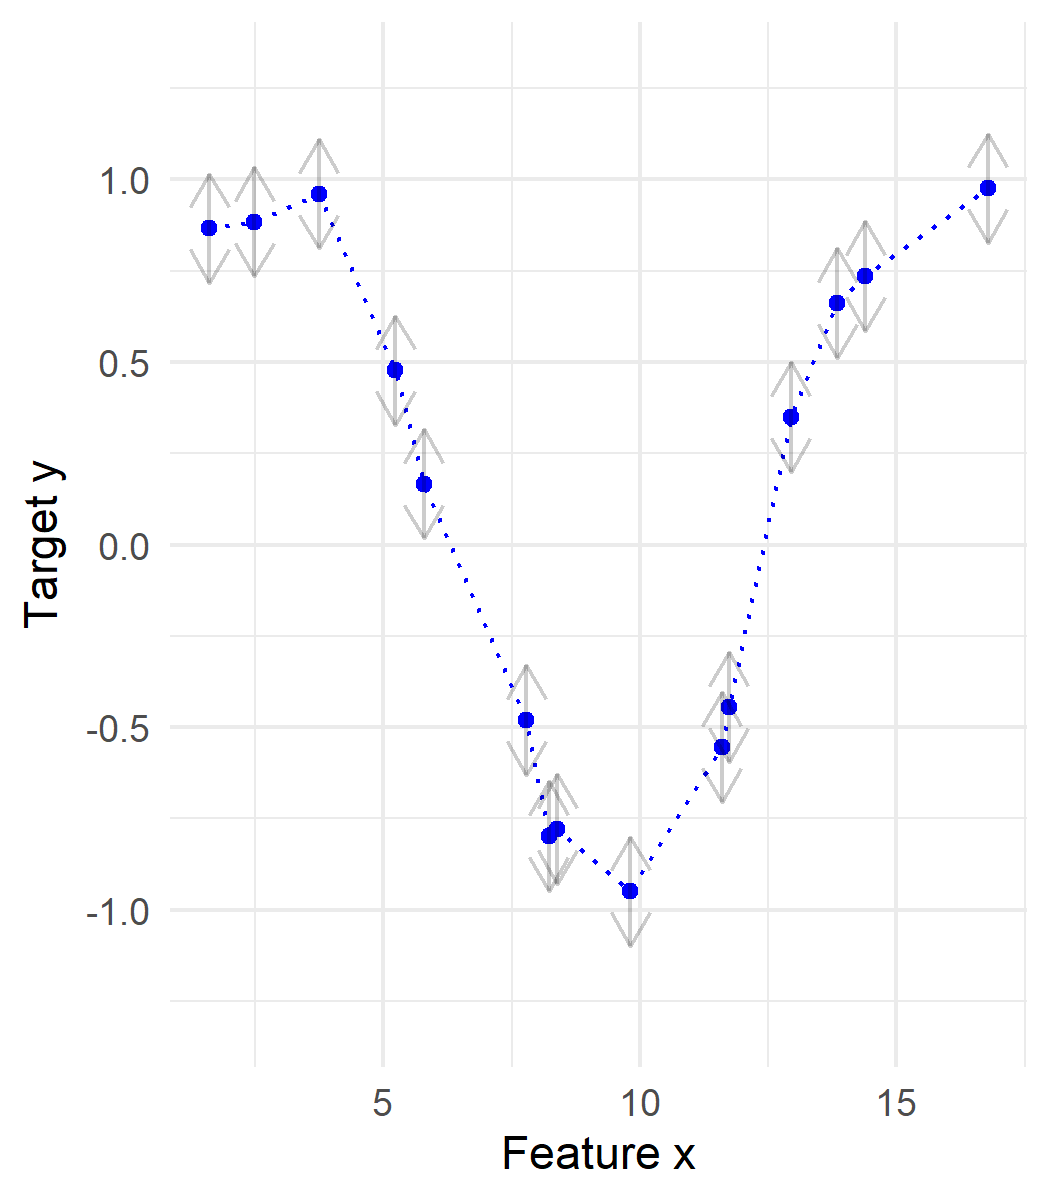
\includegraphics[width=\textwidth]{figure/fig-gb-concept-2.png}
\end{center}

\end{columns}
\end{footnotesize}
\end{vbframe}

\begin{vbframe}{Gradient boosting}

\textbf{Aim:} Define a movement in function space so we can push our current function towards the data points.

\vspace*{0.1cm}
\textbf{Given:} Regression problem with one feature $x$ and target variable $y$.

\vspace*{0.1cm}
\textbf{Initialization:} Set all parameters to the optimal constant value (e.g., the mean of $y$ for $L2$).

\begin{figure}
  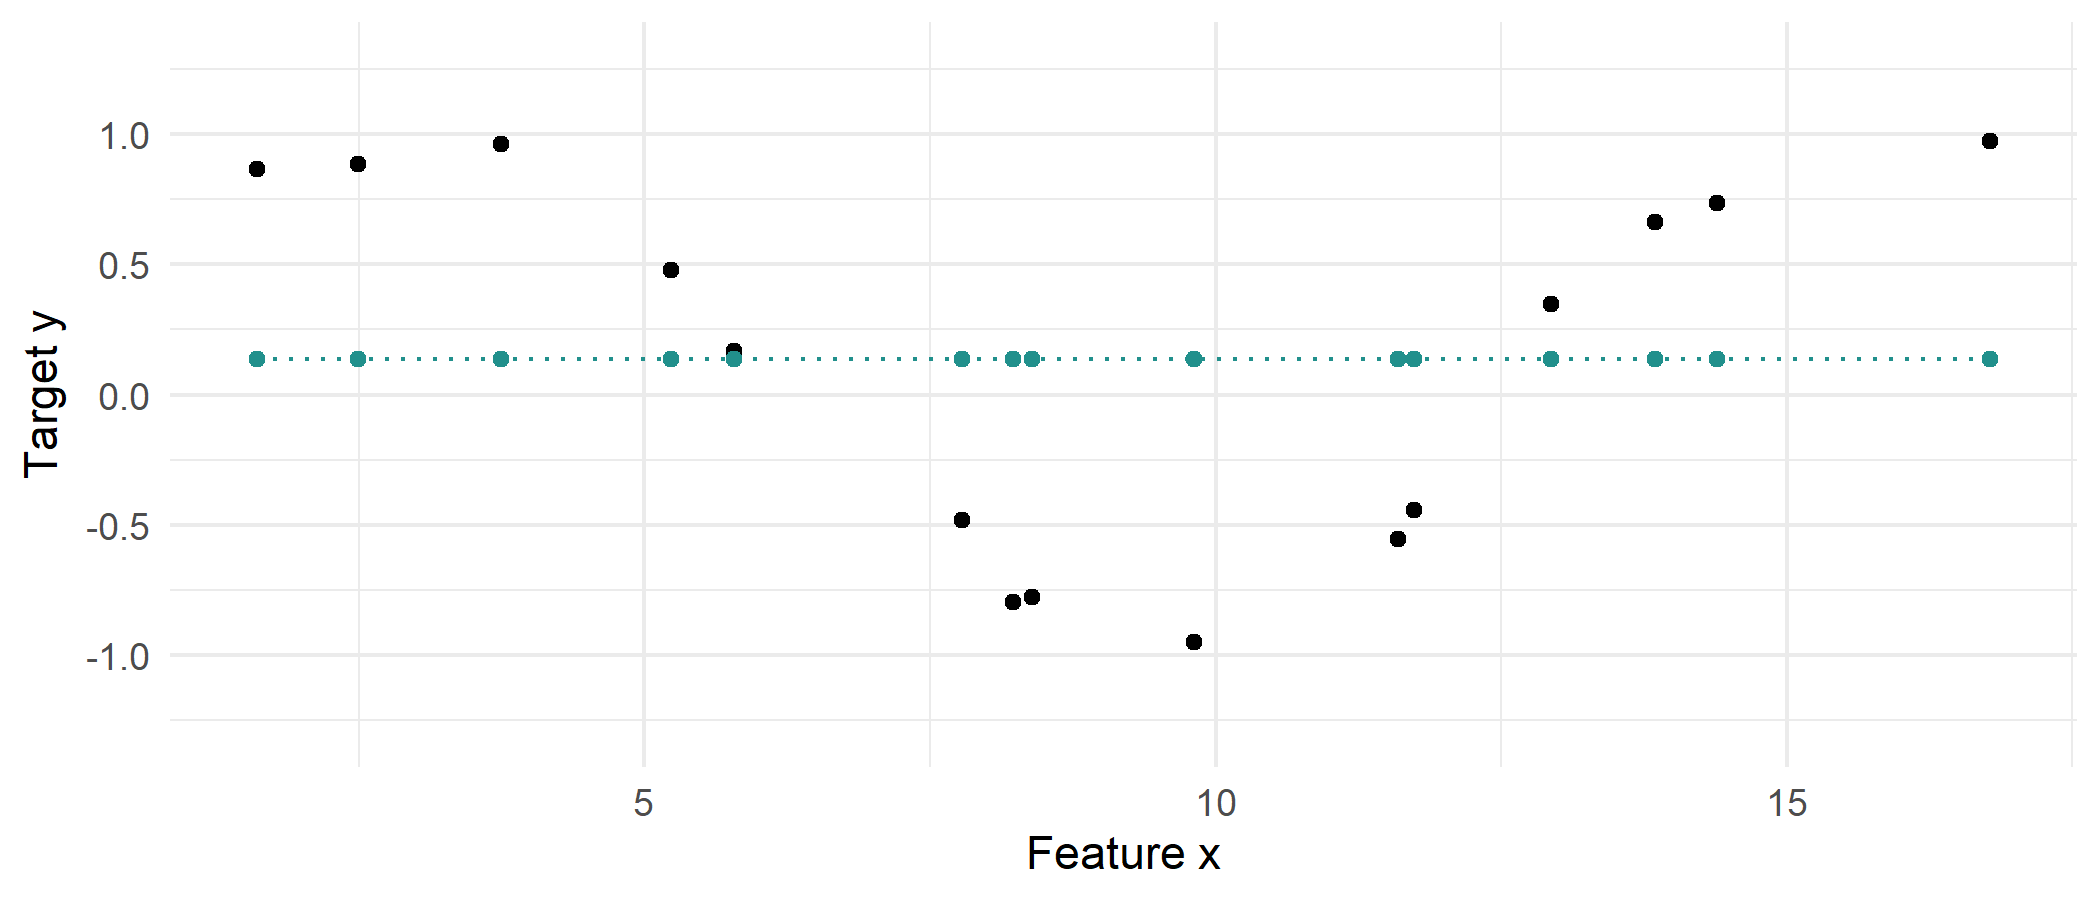
\includegraphics[width=\textwidth]{figure/fig-gb-concept-1.png}
\end{figure}



\end{vbframe}

\begin{vbframe}{Pseudo Residuals}
\begin{footnotesize}
How do we have to distort this function to move it towards the observations and drive loss down?

\vspace*{0.2cm}
We minimize the risk of such a model with gradient descent (yes, this makes no sense,
suspend all doubts for a few seconds).

So, we calculate the gradient at a point of the parameter space, that is, the derivative w.r.t. each component of the parameter vector (which is 0 for all terms with $i \neq j$):
% \footnote{The gradient of all terms with $i \neq j$ are 0.}

$$
\tilde{r}^{(i)} = - \pd{\riske}{\fxi} = - \pd{\sum_j L(y^{(j)}, f(\xv^{(j)}))}{\fxi} = - \pd{\Lxyi}{\fxi}.
$$

\vspace*{0.5cm}

\begin{minipage}[b]{0.45\textwidth}
  \raggedright
  \textbf{Reminder:} The pseudo-residuals 
  $\tilde{r}\left( f \right)$ 
  match the usual residuals for 
  the squared loss:
  \begin{align*}
  - \pd{\Lxy}{\fx} & = - \pd{0.5(y - \fx)^2}{\fx}\\ 
                   & = y - \fx
  \end{align*}
\end{minipage}%
\begin{minipage}[b]{0.05\textwidth}
   \phantom{foo}
\end{minipage}
\begin{minipage}[b]{0.45\textwidth}
  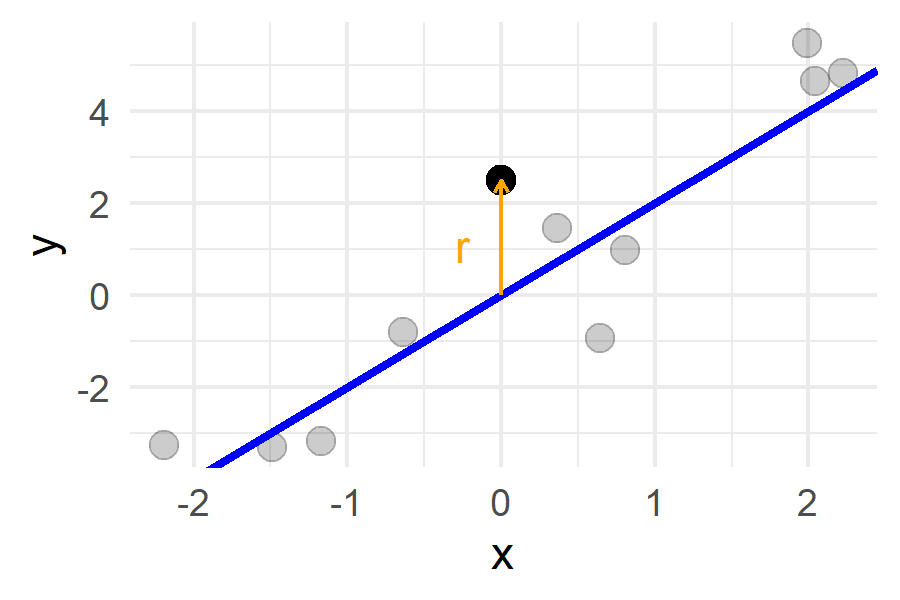
\includegraphics[width=0.9\textwidth]{figure/pseudo_residual_1.png}
\end{minipage}

\end{footnotesize}

\end{vbframe}

\begin{vbframe}{Boosting as Gradient Descent}

%\begin{footnotesize}
\vspace*{0.2cm}
Combining this with the iterative additive procedure
of \enquote{forward stagewise modeling}, we are at the spot $\fmd$ during minimization.
At this point, we now calculate the direction of the negative gradient or also called pseudo-residuals $\rmi$:

$$ \rmi = -\left[\pd{\Lxyi}{f(\xi)}\right]_{f=\fmd} $$

\lz

The gradient descent update for each vector component of $f$ is:

$$
  \fm (\xi) =  \fmd (\xi) - \alpha \pd{\Lxyi}{\fmd (\xi)}.
$$

This tells us how we could \enquote{nudge} our whole function $f$ in the direction of the data to
reduce its empirical risk.

%\end{footnotesize}
\end{vbframe}


\begin{vbframe}{Gradient boosting}

\textbf{Iteration 1:}

Let's move our function $\fxi$ a fraction towards the pseudo-residuals with a learning rate of $\alpha = 0.6$.


\begin{figure}
  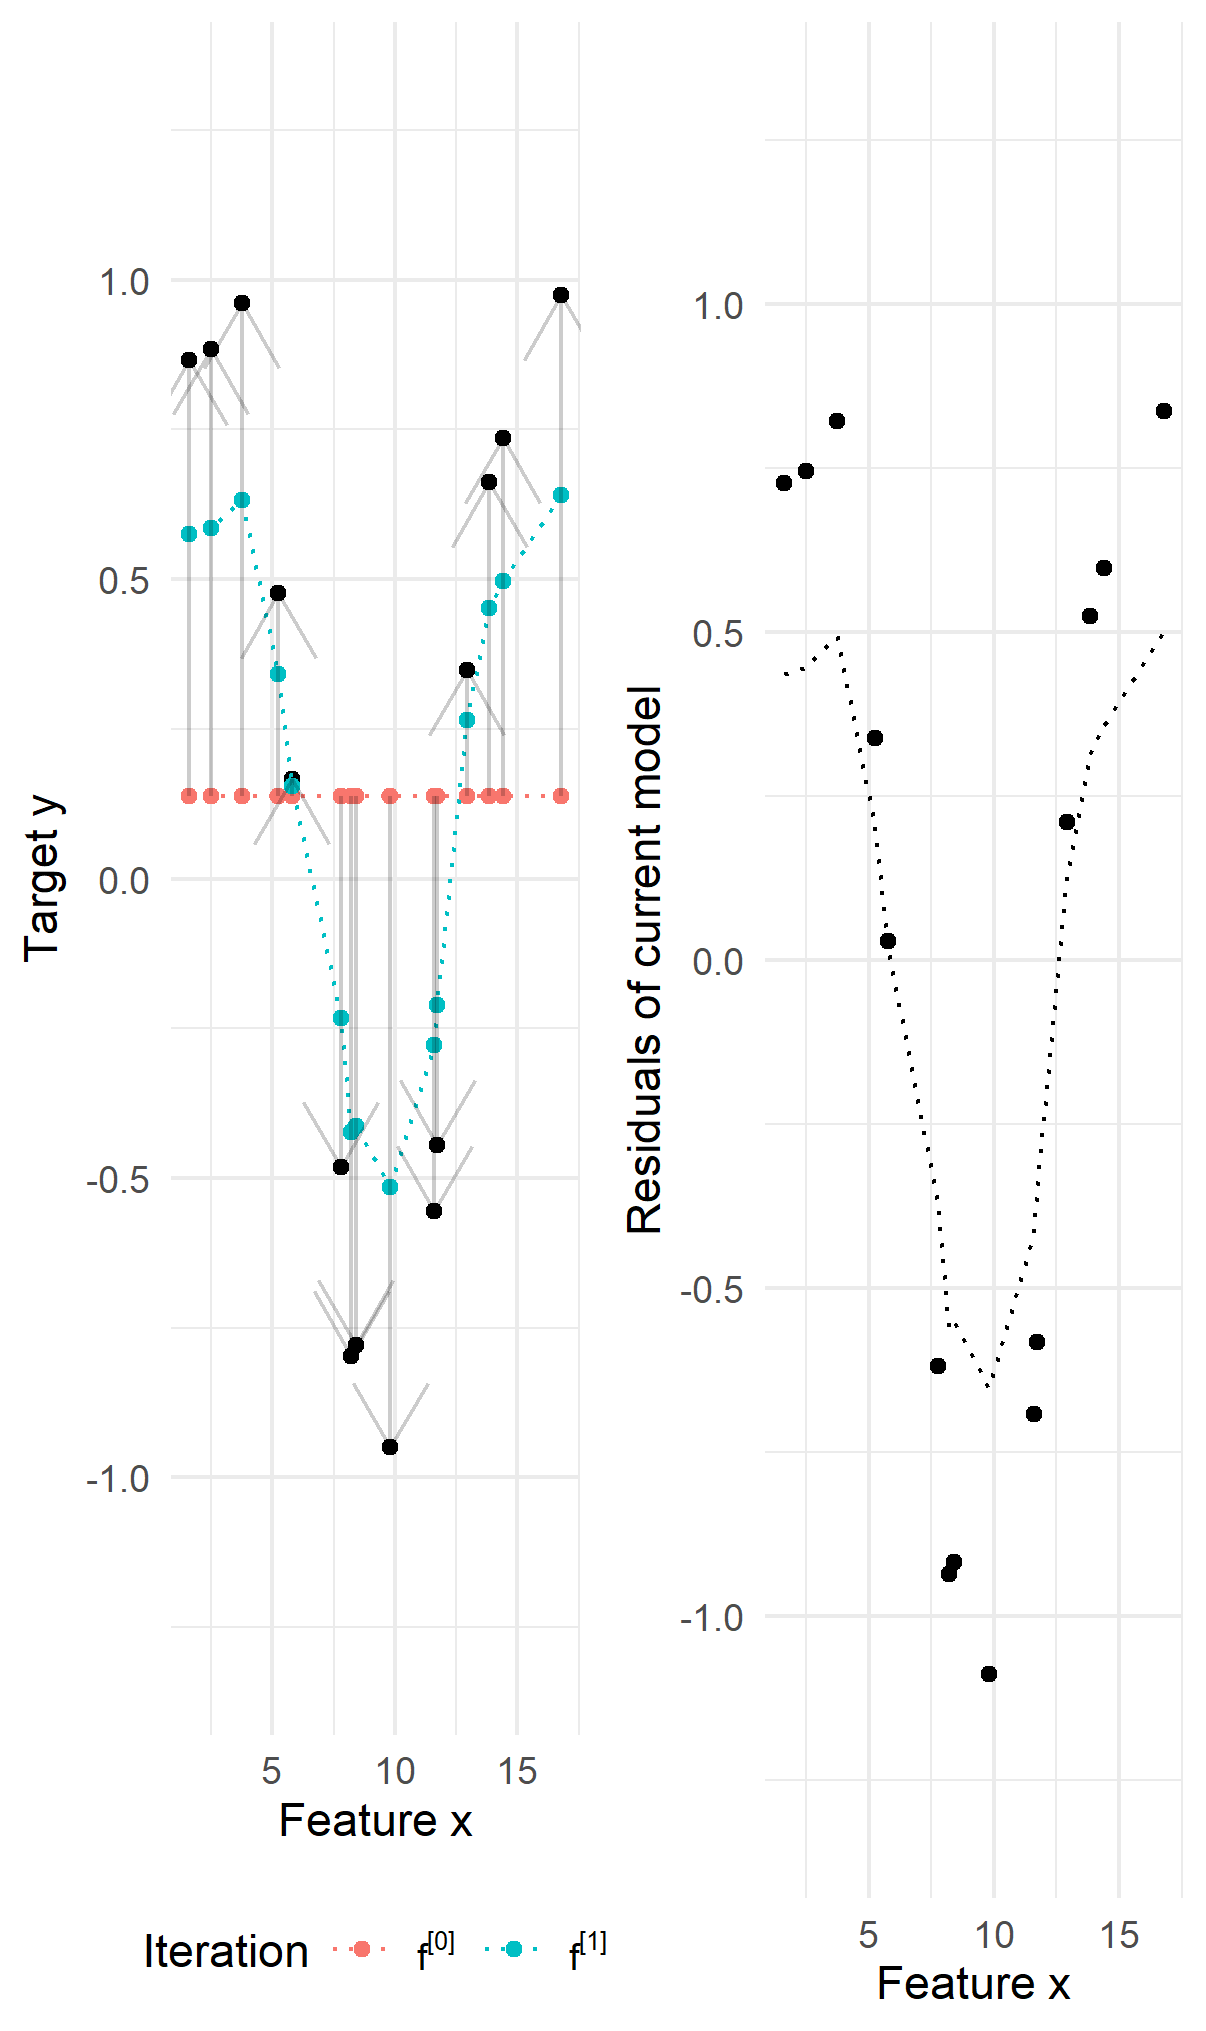
\includegraphics[width=\textwidth]{figure/fig-gb-concept-pseudo-resi-1.png}
\end{figure}

\framebreak

\textbf{Iteration 2:}

Let's move our function $\fxi$ a fraction towards the pseudo-residuals with a learning rate of $\alpha = 0.6$.


\begin{figure}
  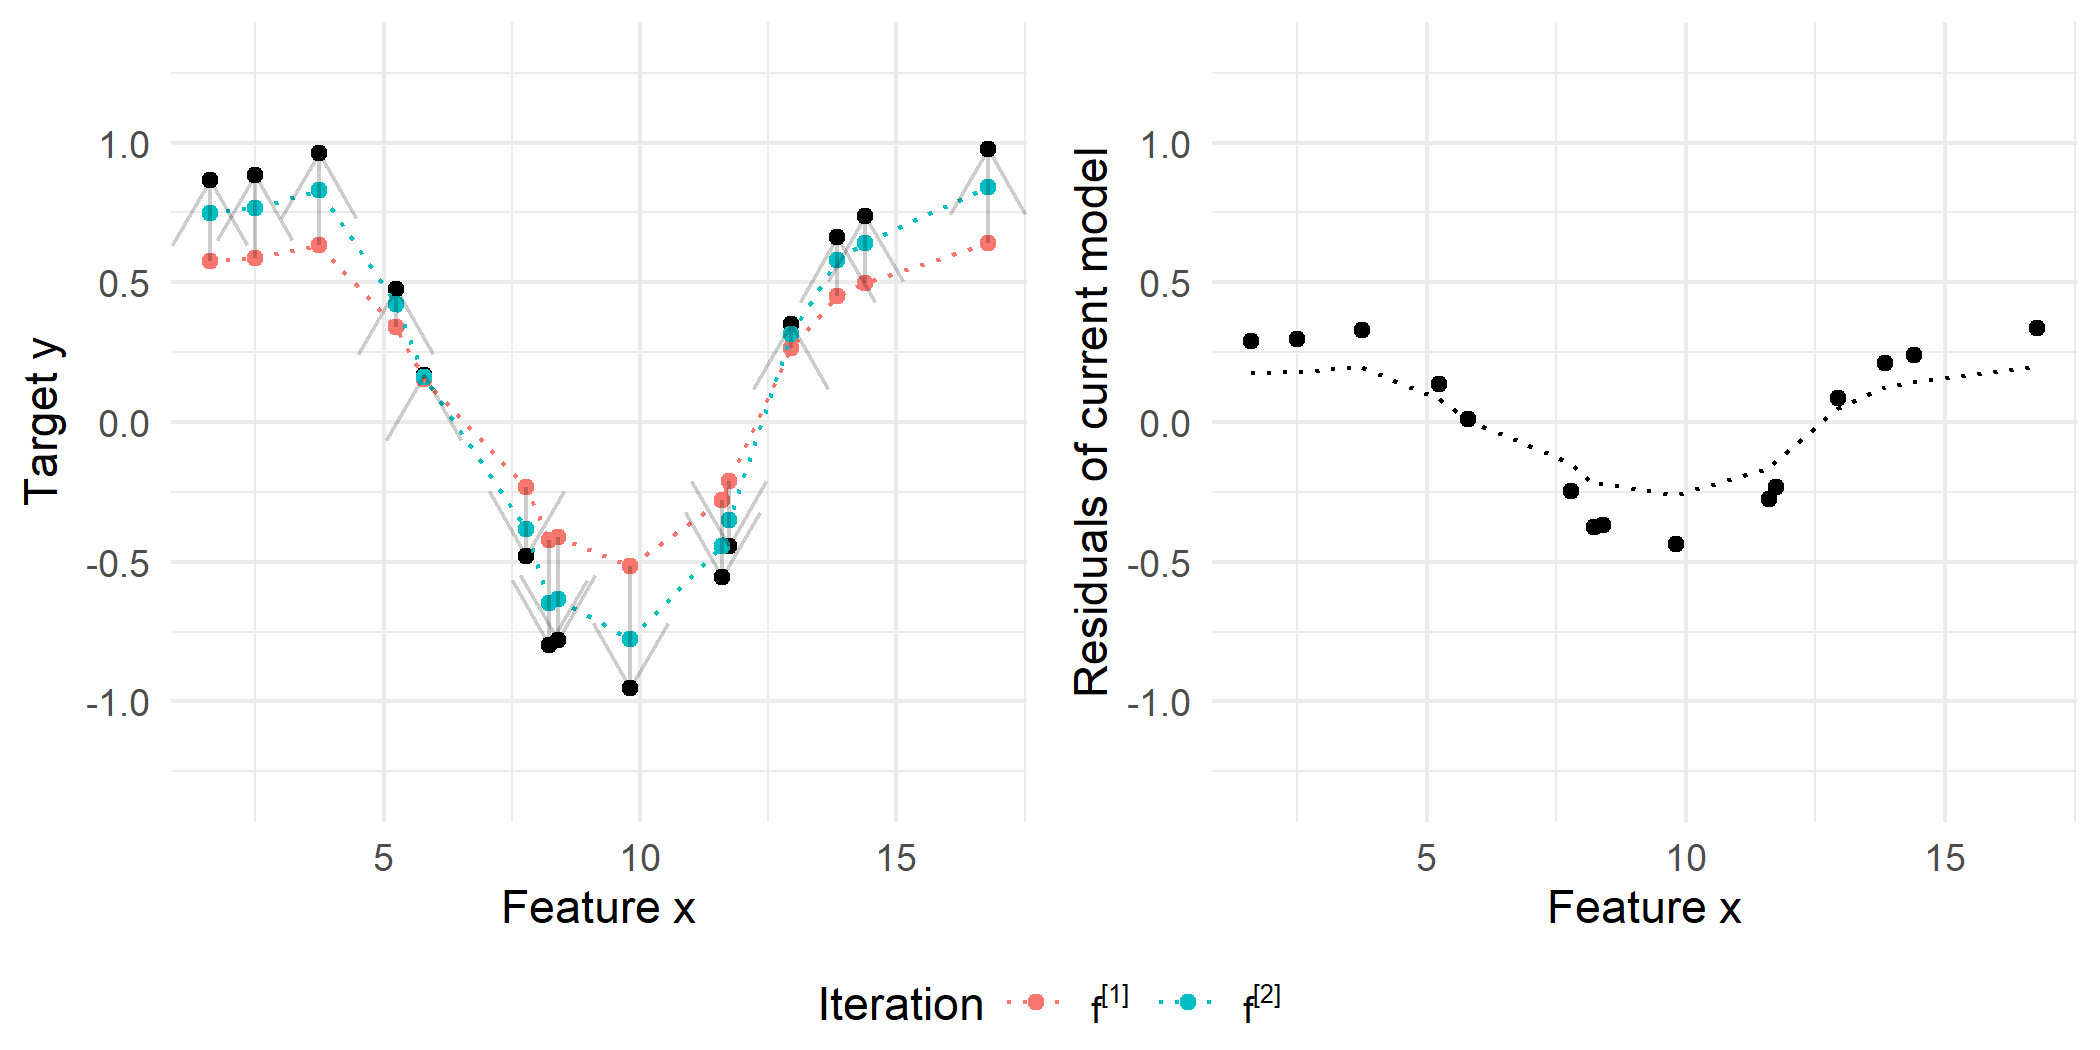
\includegraphics[width=\textwidth]{figure/fig-gb-concept-pseudo-resi-2.png}
\end{figure}

\framebreak
\begin{footnotesize}
% We find our $\betam$ by minimizing with line search:

% $$
  % \betam = \argmin_{\beta} \sumin L(\yi, \fmdh(x) + \beta b(x, \thetamh)),
% $$

% where $h(x, \thetam) = \rmm$.

% \lz

%What is the point of doing all this? 
To parameterize a model in this way is pointless,
as it just memorizes the instances of the training data.

\vspace*{0.3cm}


So, we restrict our additive components to $b\left(\xv, \thetam\right) \in \mathcal{B}$.

% \framebreak

The pseudo-residuals are calculated exactly as stated above,
then we fit a simple model $b(\xv, \thetam)$ to them:
$$ \thetamh = \argmin_{\bm{\theta}} \sum_{i=1}^n \left(\rmi - b(\xi, \bm{\theta})\right)^2. $$

\lz

\begin{columns}
\column{5cm}
So, evaluated on the training data,
our $b(\xv, \thetam)$ corresponds as closely as possible to the negative
loss function gradient and generalizes over the whole space.


\column{5cm}
\vspace*{-1cm}
\begin{figure}[th]
  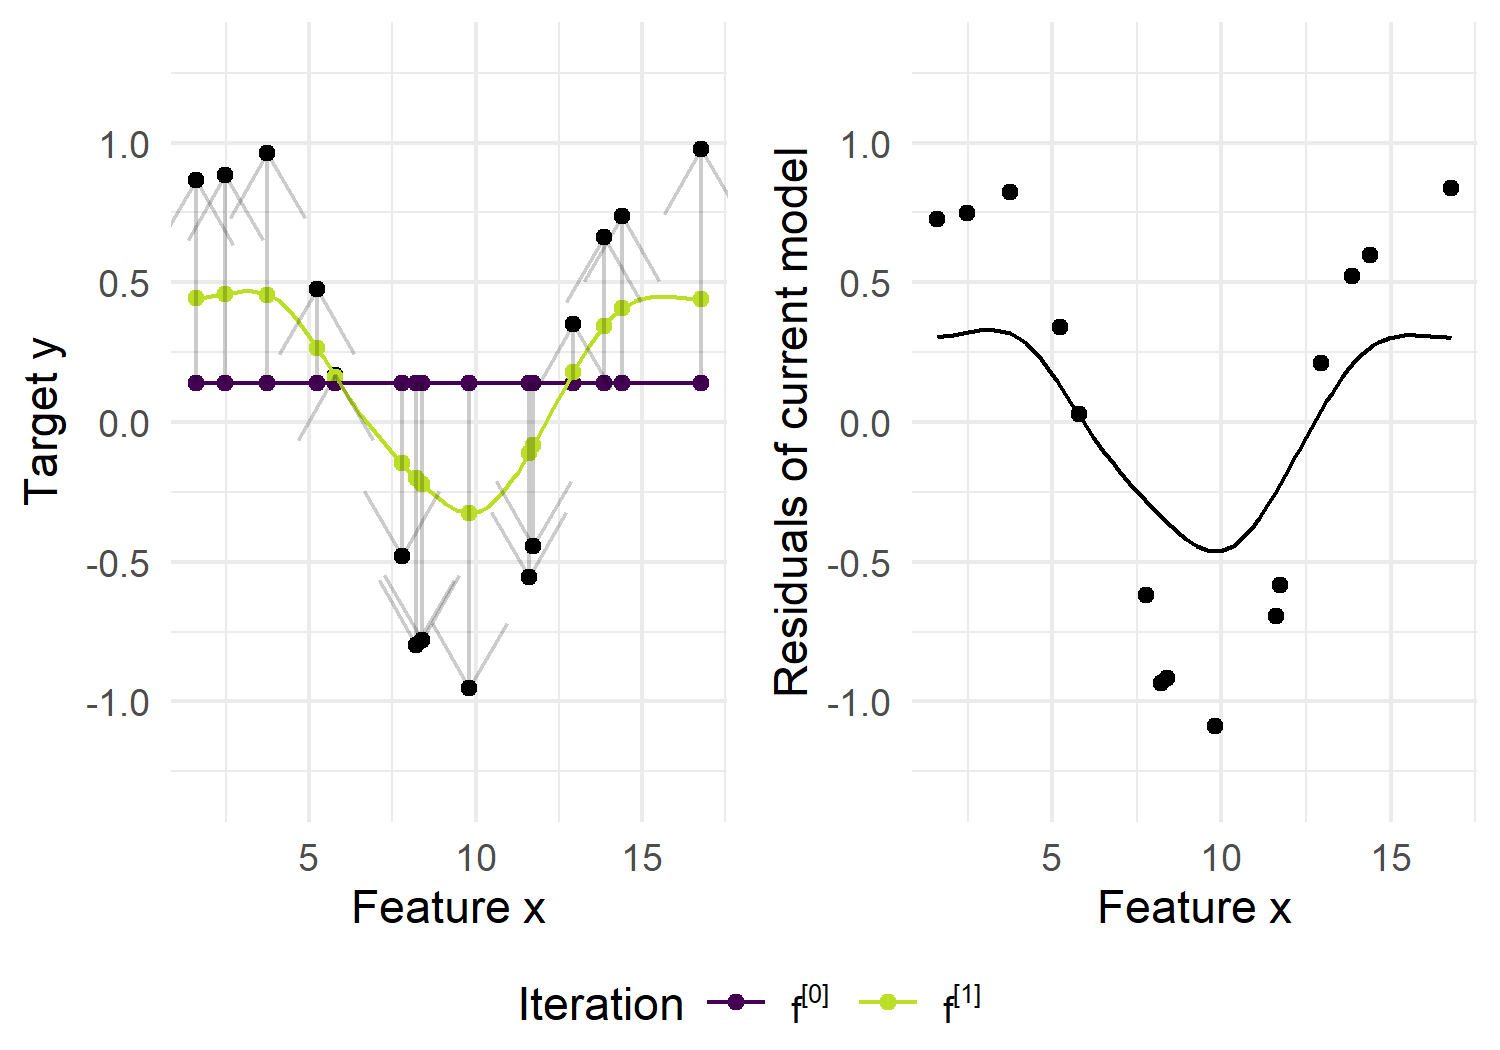
\includegraphics[width=\textwidth]{figure/fig-gb-concept-idea.png}
\end{figure}


\end{columns}
\end{footnotesize}

\framebreak
\begin{footnotesize}
\textbf{In a nutshell}: One boosting iteration is exactly one approximated gradient descent step in function space,
which minimizes the empirical risk as much as possible.


\vspace*{0.1cm}
\textbf{Iteration 1:}
\begin{figure}
  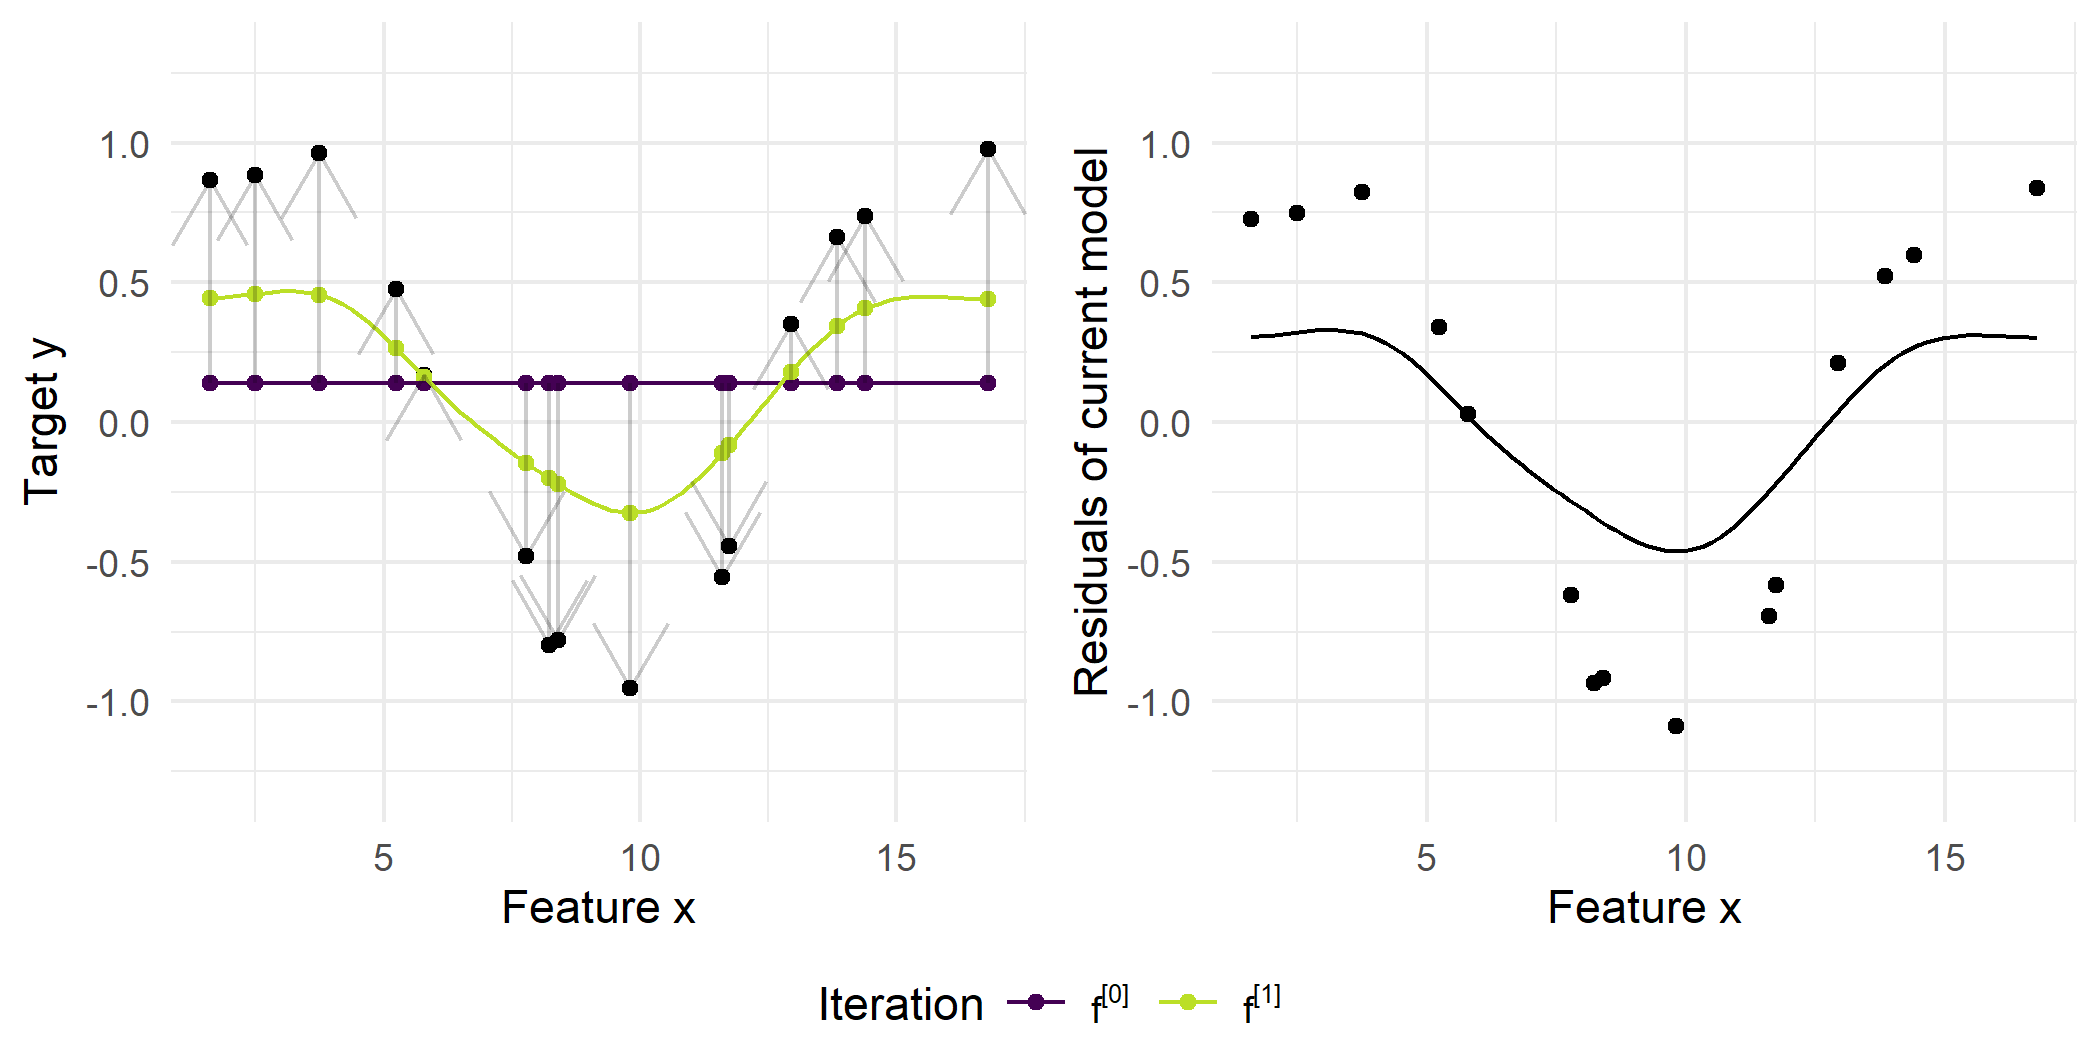
\includegraphics[width=\textwidth]{figure/fig-gb-concept-idea-1.png}
\end{figure}
\end{footnotesize}
\framebreak
\begin{footnotesize}
Instead of moving the function values for each observation by a fraction closer to the observed data, we fit a regression base learner to the pseudo-residuals (right plot). 


\vspace*{0.1cm}
\textbf{Iteration 2:}
\begin{figure}
  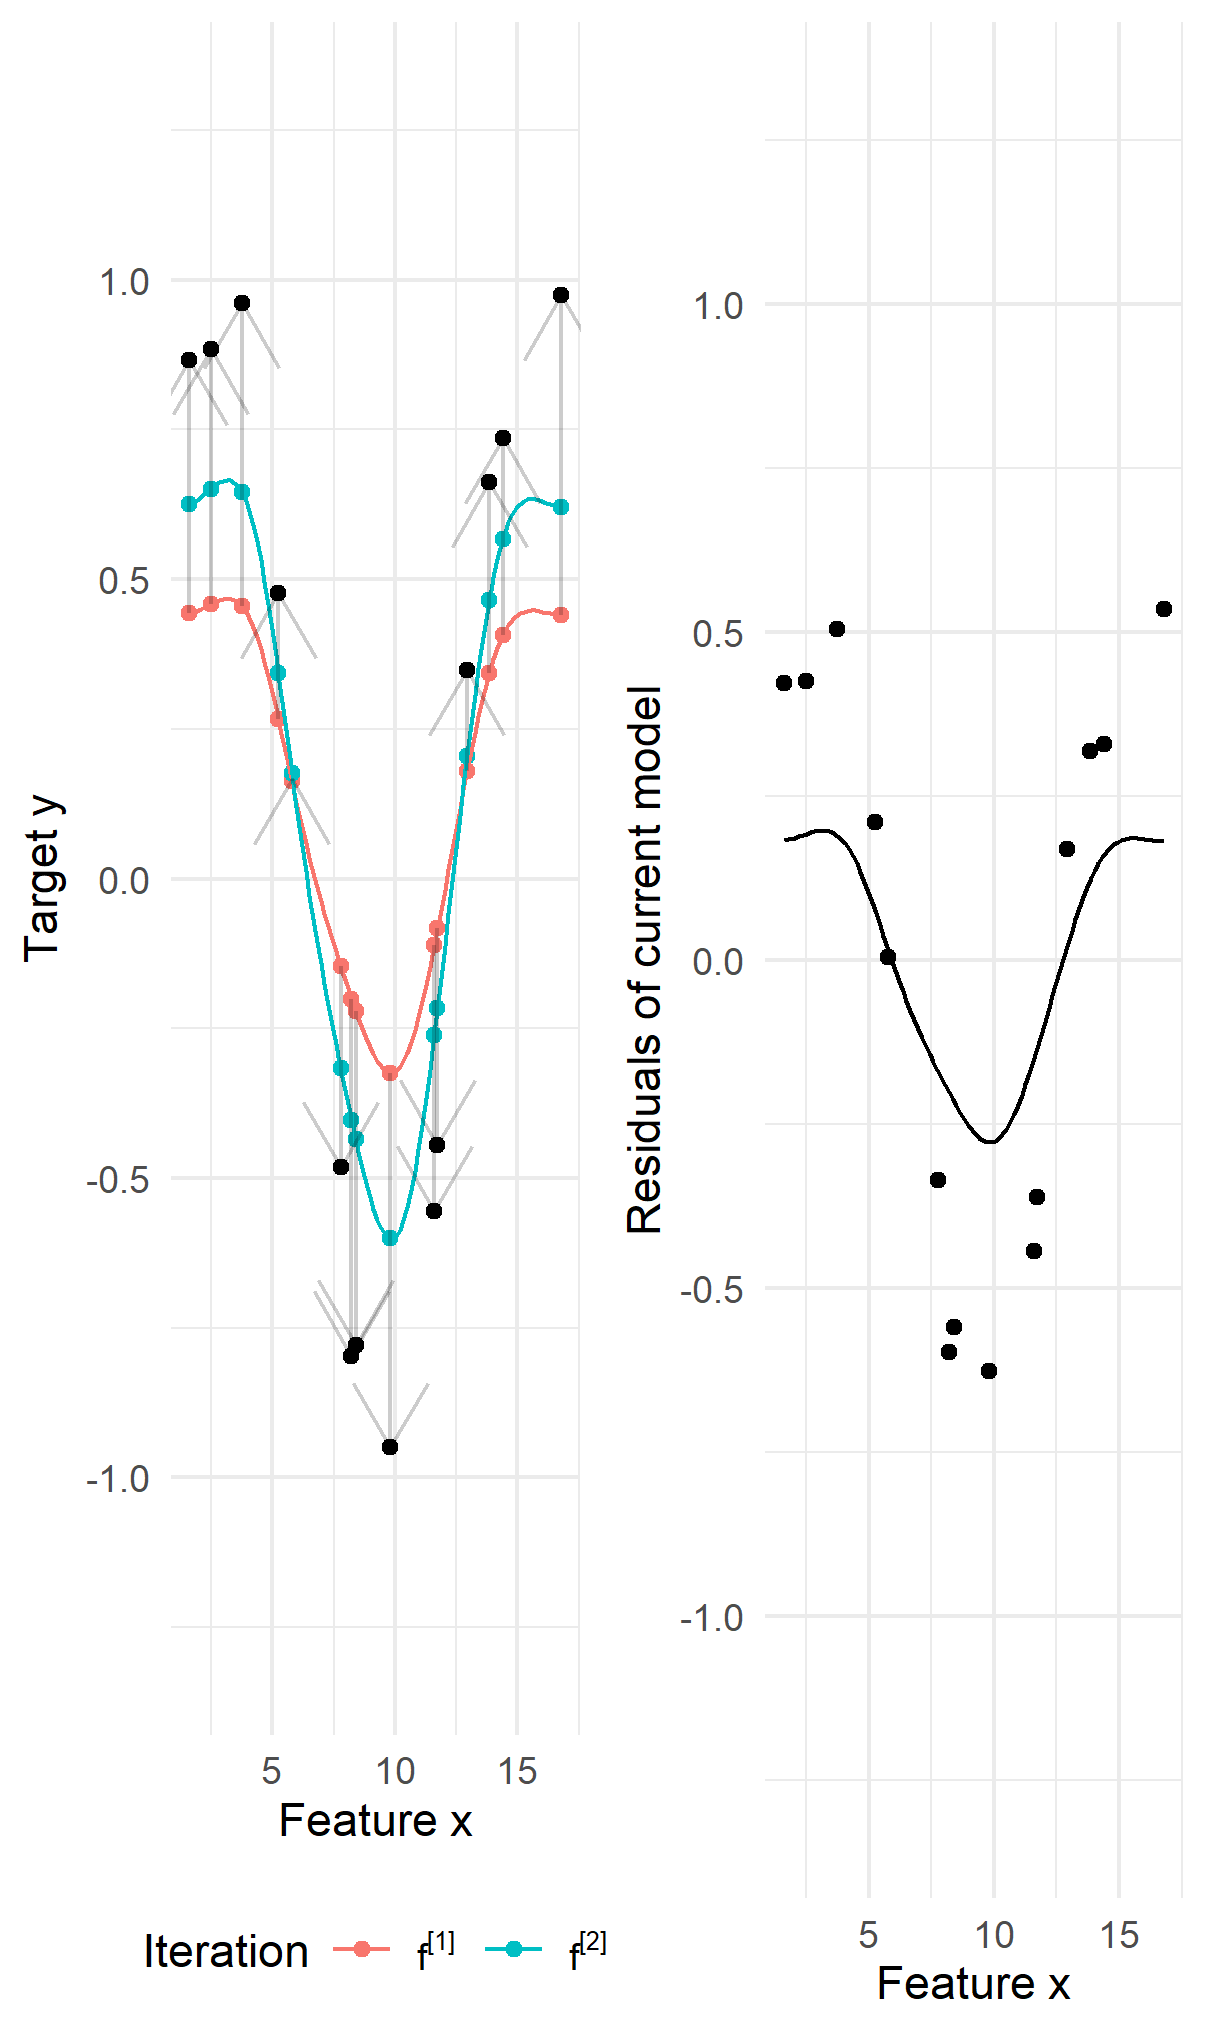
\includegraphics[width=\textwidth]{figure/fig-gb-concept-idea-2.png}
\end{figure}
\end{footnotesize}
\framebreak
\begin{footnotesize}
This base learner is then added to the current state of the ensemble weighted by the learning rate (here: $\alpha = 0.4$) and for the next iteration again the pseudo-residuals of the adapted ensemble are calculated and a base learner is fitted to them.


\vspace*{0.1cm}
\textbf{Iteration 3:}
\begin{figure}
  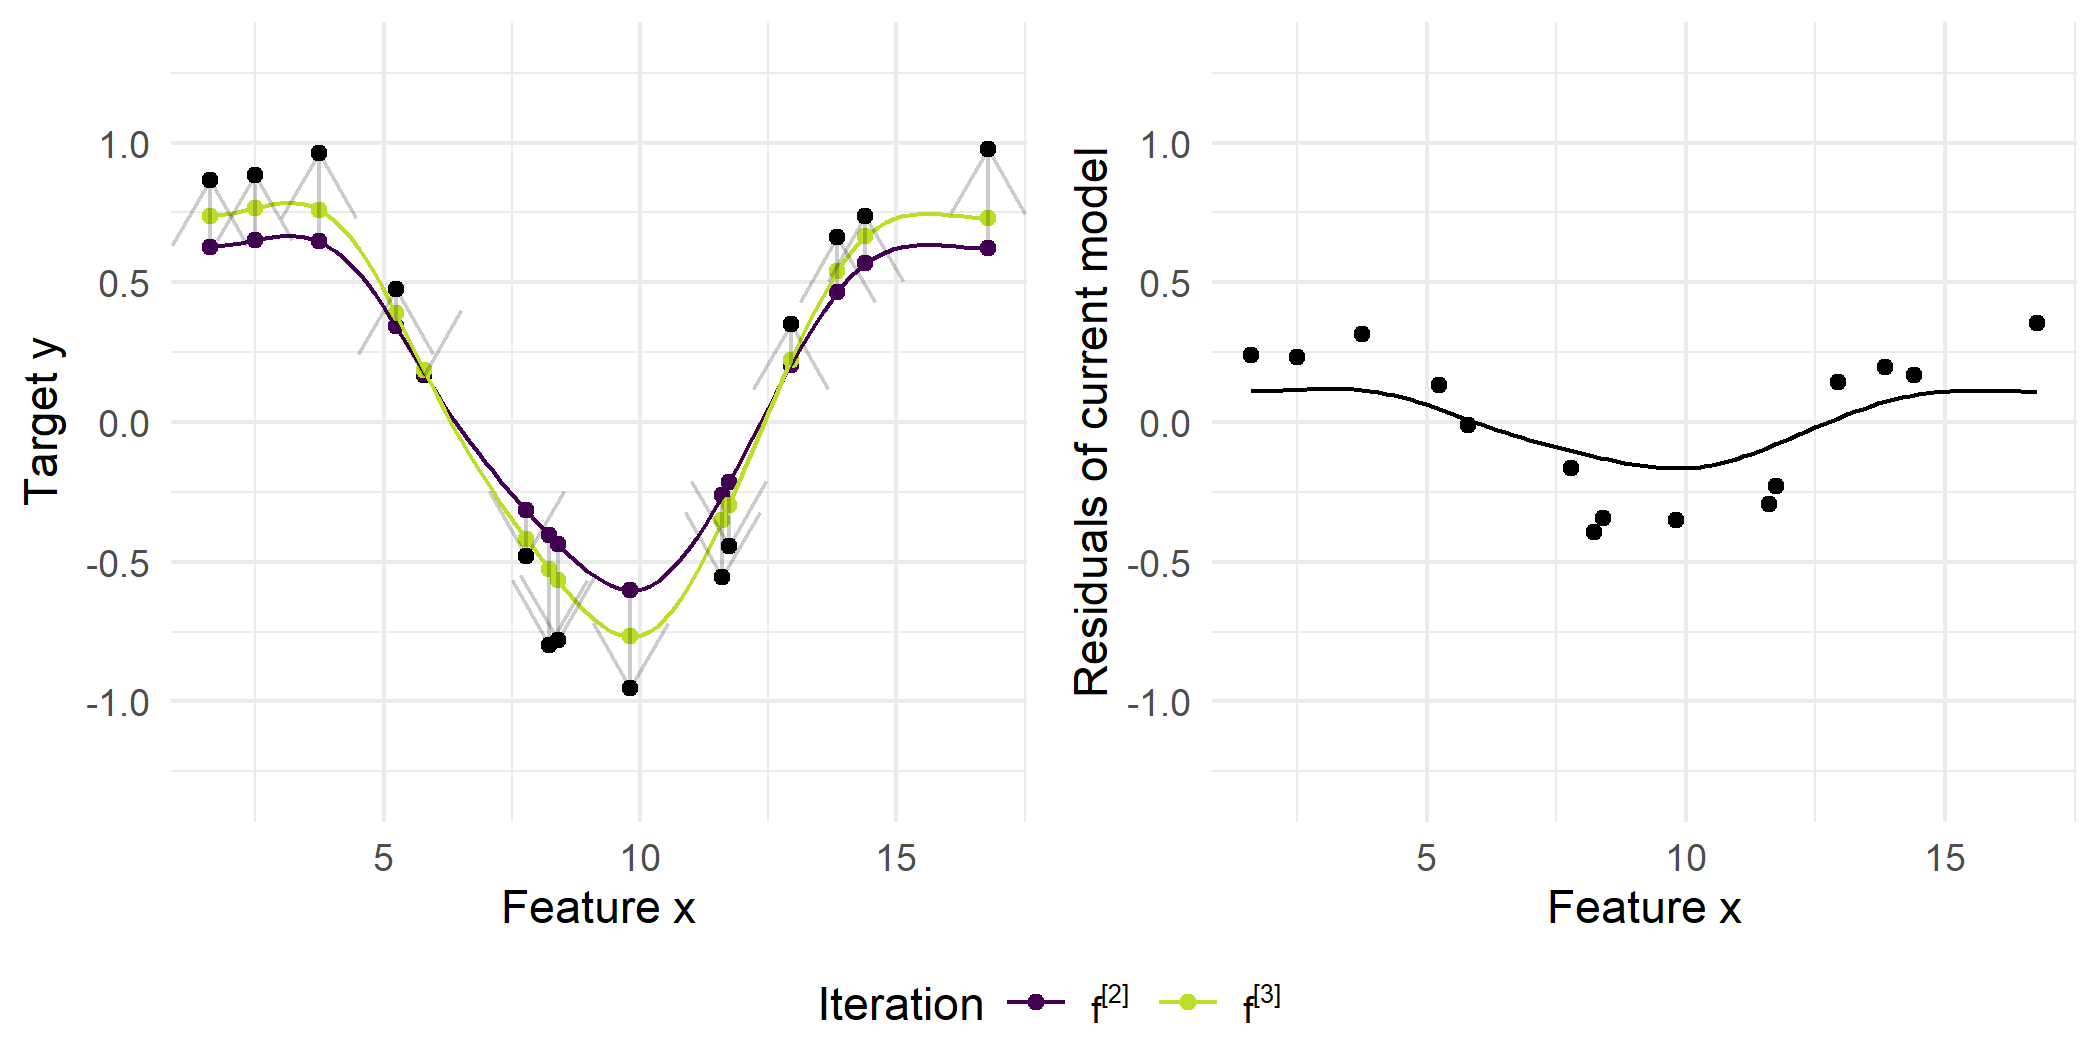
\includegraphics[width=\textwidth]{figure/fig-gb-concept-idea-3.png}
\end{figure}

% \begin{footnotesize}
% This procedure is continued stepwise until the boosting algorithm terminates.
% \end{footnotesize}
\end{footnotesize}
\end{vbframe}
%% Combining this with the iterative additive procedure
%% of \enquote{forward stagewise modelling}, we are at the spot $\fmd$ during minimization.
%% At this point, we now calculate the direction of the negative gradient:
%%
%% $$ \rmi = -\left[\pd{\Lxyi}{f(\xi)}\right]_{f=\fmd} $$
%%
%% We will call these $\rmi$ \textbf{pseudo residuals}. For squared loss they match the usual residuals
%%
%%
%% $$
%% - \pd{\Lxy}{\fx} = - \pd{0.5(y - \fx)^2}{\fx} = y - \fx
%% $$
%%
%%
%% \framebreak
%%
%% % We find our $\betam$ by minimizing with line search:
%%
%% % $$
%%   % \betam = \argmin_{\beta} \sumin L(\yi, \fmdh(x) + \beta b(x, \thetamh)),
%% % $$
%%
%% % where $h(x, \thetam) = \rmm$.
%%
%% % \lz
%%
%% What is the point in doing all this? A model parameterized in this way is senseless,
%% as it is just memorizing the instances of the training data...?
%%
%% \lz
%%
%% So, we restrict our additive components to $b\left(x, \thetam\right) \in \mathcal{B}$.
%%
%% % \framebreak
%%
%% The pseudo-residuals are calculated exactly as stated above,
%% then we fit a regression model $b(\bm{x}, \thetam)$ to them:
%% $$ \thetamh = \argmin_{\thetab} \sum_{i=1}^n (\rmi - b(\xi, \thetab))^2 $$
%% So, evaluated on the training data,
%% our $b(x, \thetam)$ corresponds as closely as possible to the negative
%% loss function gradient and generalizes to the whole space.
%%
%% \lz
%%
%% \textbf{In a nutshell}: One boosting iteration is exactly one approximated gradient step in function space,
%% which minimizes the empirical risk as much as possible.
%%
%% \end{vbframe}

\begin{vbframe}{Gradient boosting algorithm}

\begin{algorithm}[H]
  \begin{footnotesize}
  \begin{center}
  \caption{Gradient Boosting Algorithm.}
    \begin{algorithmic}[1]
      \State Initialize $\hat{f}^{[0]}(\xv) = \argmin_{\bm{\theta}} \sumin L(\yi, b(\xi, \bm{\theta}))$
      %\State Set the learning rate $\beta$ to a small constant value
      \For{$m = 1 \to M$}
          \State For all $i$: $\rmi = -\left[\pd{\Lxyi}{\fxi}\right]_{f=\fmdh}$
        \State Fit a regression base learner to the pseudo-residuals $\rmi$:
        \State $\thetamh = \argmin \limits_{\bm{\theta}} \sumin (\rmi - b(\xi, \bm{\theta}))^2$
        %\State Line search: $\betamh = \argmin_{\beta} \sumin L(\yi, \fmd(\xv) + \beta b(\xv, \thetamh))$
        \State Set $\alpha^{[m]}$ to $\alpha$ being a small constant value or via line search
        \State Update $\fmh(\xv) = \fmdh(\xv) + \alpha^{[m]} b(\xv, \thetamh)$
      \EndFor
      \State Output $\fh(\xv) = \hat{f}^{[M]}(\xv)$
    \end{algorithmic}
    \end{center}
    \end{footnotesize}
\end{algorithm}


Note that we also initialize the model in a loss-optimal manner. %Also, the constant learning rate can be replaced by a line-search, however a small constant learning rate is commonly used.

\end{vbframe}

\begin{vbframe}{Line Search}
The learning rate in gradient boosting influences how fast the algorithm converges. 
Although a small constant learning rate is commonly used in practice, it can also be replaced by a line search.\\\lz
Line search is an iterative approach to find a local minimum. In the case of setting the learning rate, the following one-dimensional optimization problem has to be solved:
$$\hat{\alpha}^{[m]} = \argmin_{\alpha} \sumin L(\yi, \fmd(\xv) + \alpha b(\xv, \thetamh))$$

Optionally, an (inexact) backtracking line search can be used to find the 
$\alpha^{[m]}$ that minimizes the above equation.

\end{vbframe}

\endlecture
\end{document}

